\chapter{Implementación}

\section{Diseño del Sofware}

\noindent El diseño software no se ha orientado a crear un programa funcional para ser empleado por un usuario, sino que tiene como función entrenar los modelos probados y recabar los resultados oportunos del proceso de experimentación. Se ha utilizado el sistema de control de versiones \textit{Git} junto con \textit{GitHub}. En total se han creado dos repositorios:

\begin{enumerate}
    \item Un repositorio con la planificación y elaboración de la memoria junto con los scripts para el preprocesamiento de los datos: \url{https://github.com/alejbormeg/TFG-LandmarkDetectionAndCNNAnalysis}
    \item Un \textit{fork} a partir del repositorio principal del paper, dónde se han elaborado todas las adaptaciones a nuestro problema: \url{https://github.com/alejbormeg/3FabRec/tree/master}
\end{enumerate}

\medskip

\noindent Se ha programado un \textit{notebook} de Jupyter independiente al proyecto general del framework, en el cual, se realiza el preprocesamiento de los datos, la identificación de las caras y la separación en conjunto de entrenamiento y test. El fichero se denomina \textit{Make\_crop\_split\_database.ipynb}. También se creó un fichero para la generación de diagramas de cajas y test de contraste de hipótesis denominado \textit{Boxplot\_hypothesis\_test.ipynb}.

\medskip

\noindent Por otro lado, en lo que respecta al entrenamiento y diseño de la red, partíamos de un proyecto ya elaborado minuciosamente que se ha tenido que adaptar para aceptar como entrada la nueva base de datos así como alterar ciertas partes de su entrenamiento (para poder hacer el ajuste fino del decoder por ejemplo, realizar técnicas de \textit{cross validation 5-fold}) o introducir nuevos parámetros y funciones para la obtención y manipulación de los datos, y la generación de las gráficas y tablas de resultados que se muestran. Además se tuvieron que alterar las funciones del cálculo de métricas para que tuvieran en cuenta que en todas las imágenes no necesariamente se incluían todos los landmarks, y por lo tanto que solo computasen aquellos presentes en las mismas.

\begin{figure}[!h]
    \centering
    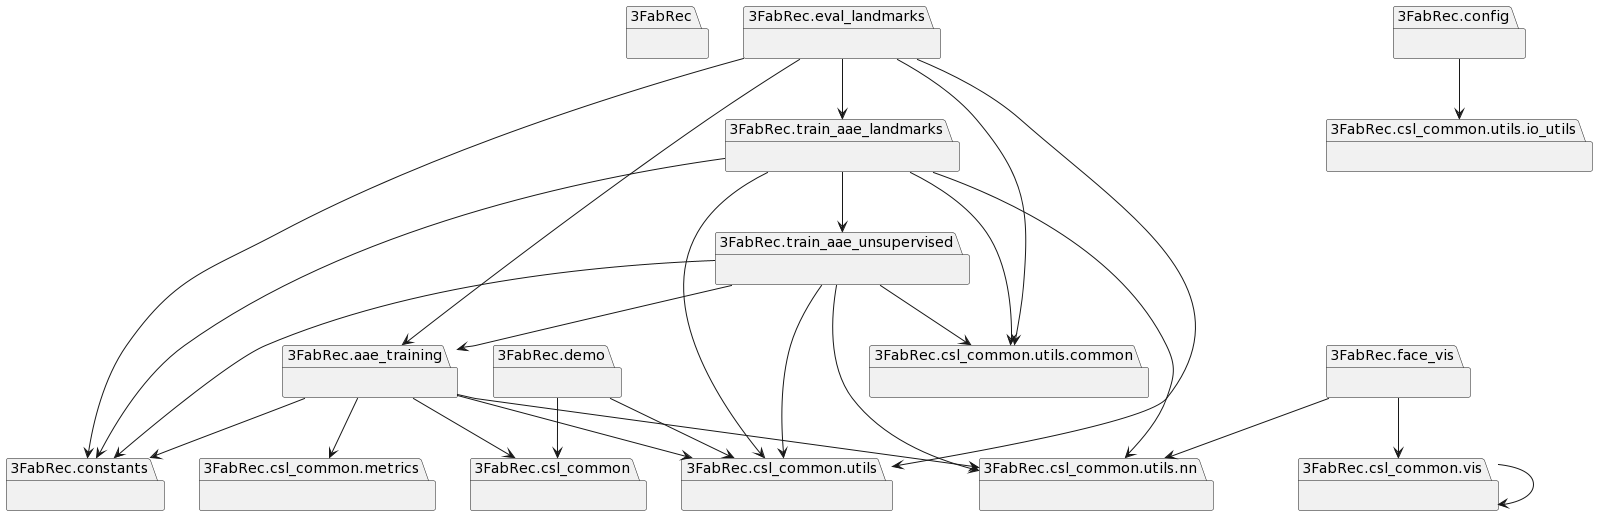
\includegraphics[width=0.99\textwidth]{img/diagrama_paquetes_1.png}
    \caption{Diagrama de paquetes del proyecto generado por \textit{pyreverse}, herramienta incluida en el paquete Pylint}
    \label{fig:Diagrama_paquetes}
\end{figure}

\medskip

\noindent La estructura de paquetes la podemos ver en la \autoref{fig:Diagrama_paquetes}. Los paquetes en color verde son los que han sido modificados o creados para este trabajo, el resto pertenecen al software original de \cite{browatzki20203fabrec}:

\begin{itemize}
    \item \textcolor{mygreen}{\textbf{3FabRec.eval\_landmarks}}: Se lleva a acabo la evaluación del modelo en el conjunto de test y se extraen las métricas. Se adapta para extraer el \textbf{RMSE} por landmark teniendo en cuenta que cada landmark puede estar no marcado en algunas imágenes.
    \item \textcolor{mygreen}{\textbf{3FabRec.train\_aae\_landmarks}}: Se lleva a cabo todo el proceso del entrenamiento supervisado del marcado de landmarks. Es el fichero que más se ha tenido que modificar, pues hemos cambiado la lógica del entrenamiento con respecto a la del framework original. Los parámetros de ejecución se encuentran en la \autoref{table:Params}.
    \item \textbf{3FabRec.train\_aae\_unsupervised}: En este paquete se lleva a cabo el entrenamiento no supervisado de la red.
    \item Los dos paquetes anteriores, a su vez se combinan en \textbf{3FabRec.aa\_training}, que encapsula toda la lógica del entrenamiento, incluyendo el aprendizaje supervisado y el no supervisado.
    \item El paquete \textbf{3FabRec.landmarks} lleva a cabo todo lo relaitvo a la manipulación de los landmarks, el cálculo de los errores asociados a los mismos, el paso de Heat maps a coordenadas y la inversa, etc... En este fichero se ha tenido que modificar el subpaquete \textcolor{mygreen}{\textbf{3FabRec.lanmarks.lmutils}} y \textcolor{mygreen}{\textbf{3FabRec.landmakrs.lmvis}}. En el caso del primero porque hemos modificado algunas funciones que calculan las métricas de error adaptándolas al problema y en el caso del segundo porque no toda la información que se mostraban en las imágenes de salida era relevante para nuestro estudio, por lo que se han eliminado los datos innecesarios.
    \item El paquete \textbf{3FabRec.constants} contiene variables globales relativas a los conjuntos de datos de entrenamiento, validación y test.
    \item El paquete \textbf{3FabRec.networks} contienen todas las redes que se emplean en la arquitectura de la red. En concreto usaremos \textbf{3FabRec.networks.aae} en la cual se encuentra la estructura general del adversarial autoencoder.
    \item El paquete \textbf{3FabRec.datasets} contiene todos los ficheros relativos a la creación de la clase \textit{Dataset} y \textit{Dataloader} para cada base de datos concreta que se emplea en el framework. Dentro de este paquete se crea el fichero \textcolor{mygreen}{\textbf{3FabRec.datasets.forense\_am}}, que se encarga de la lectura correcta de los datos de entrenamiento de la base de datos proporcionada.
\end{itemize}


\begin{figure}[!h]
    \centering
    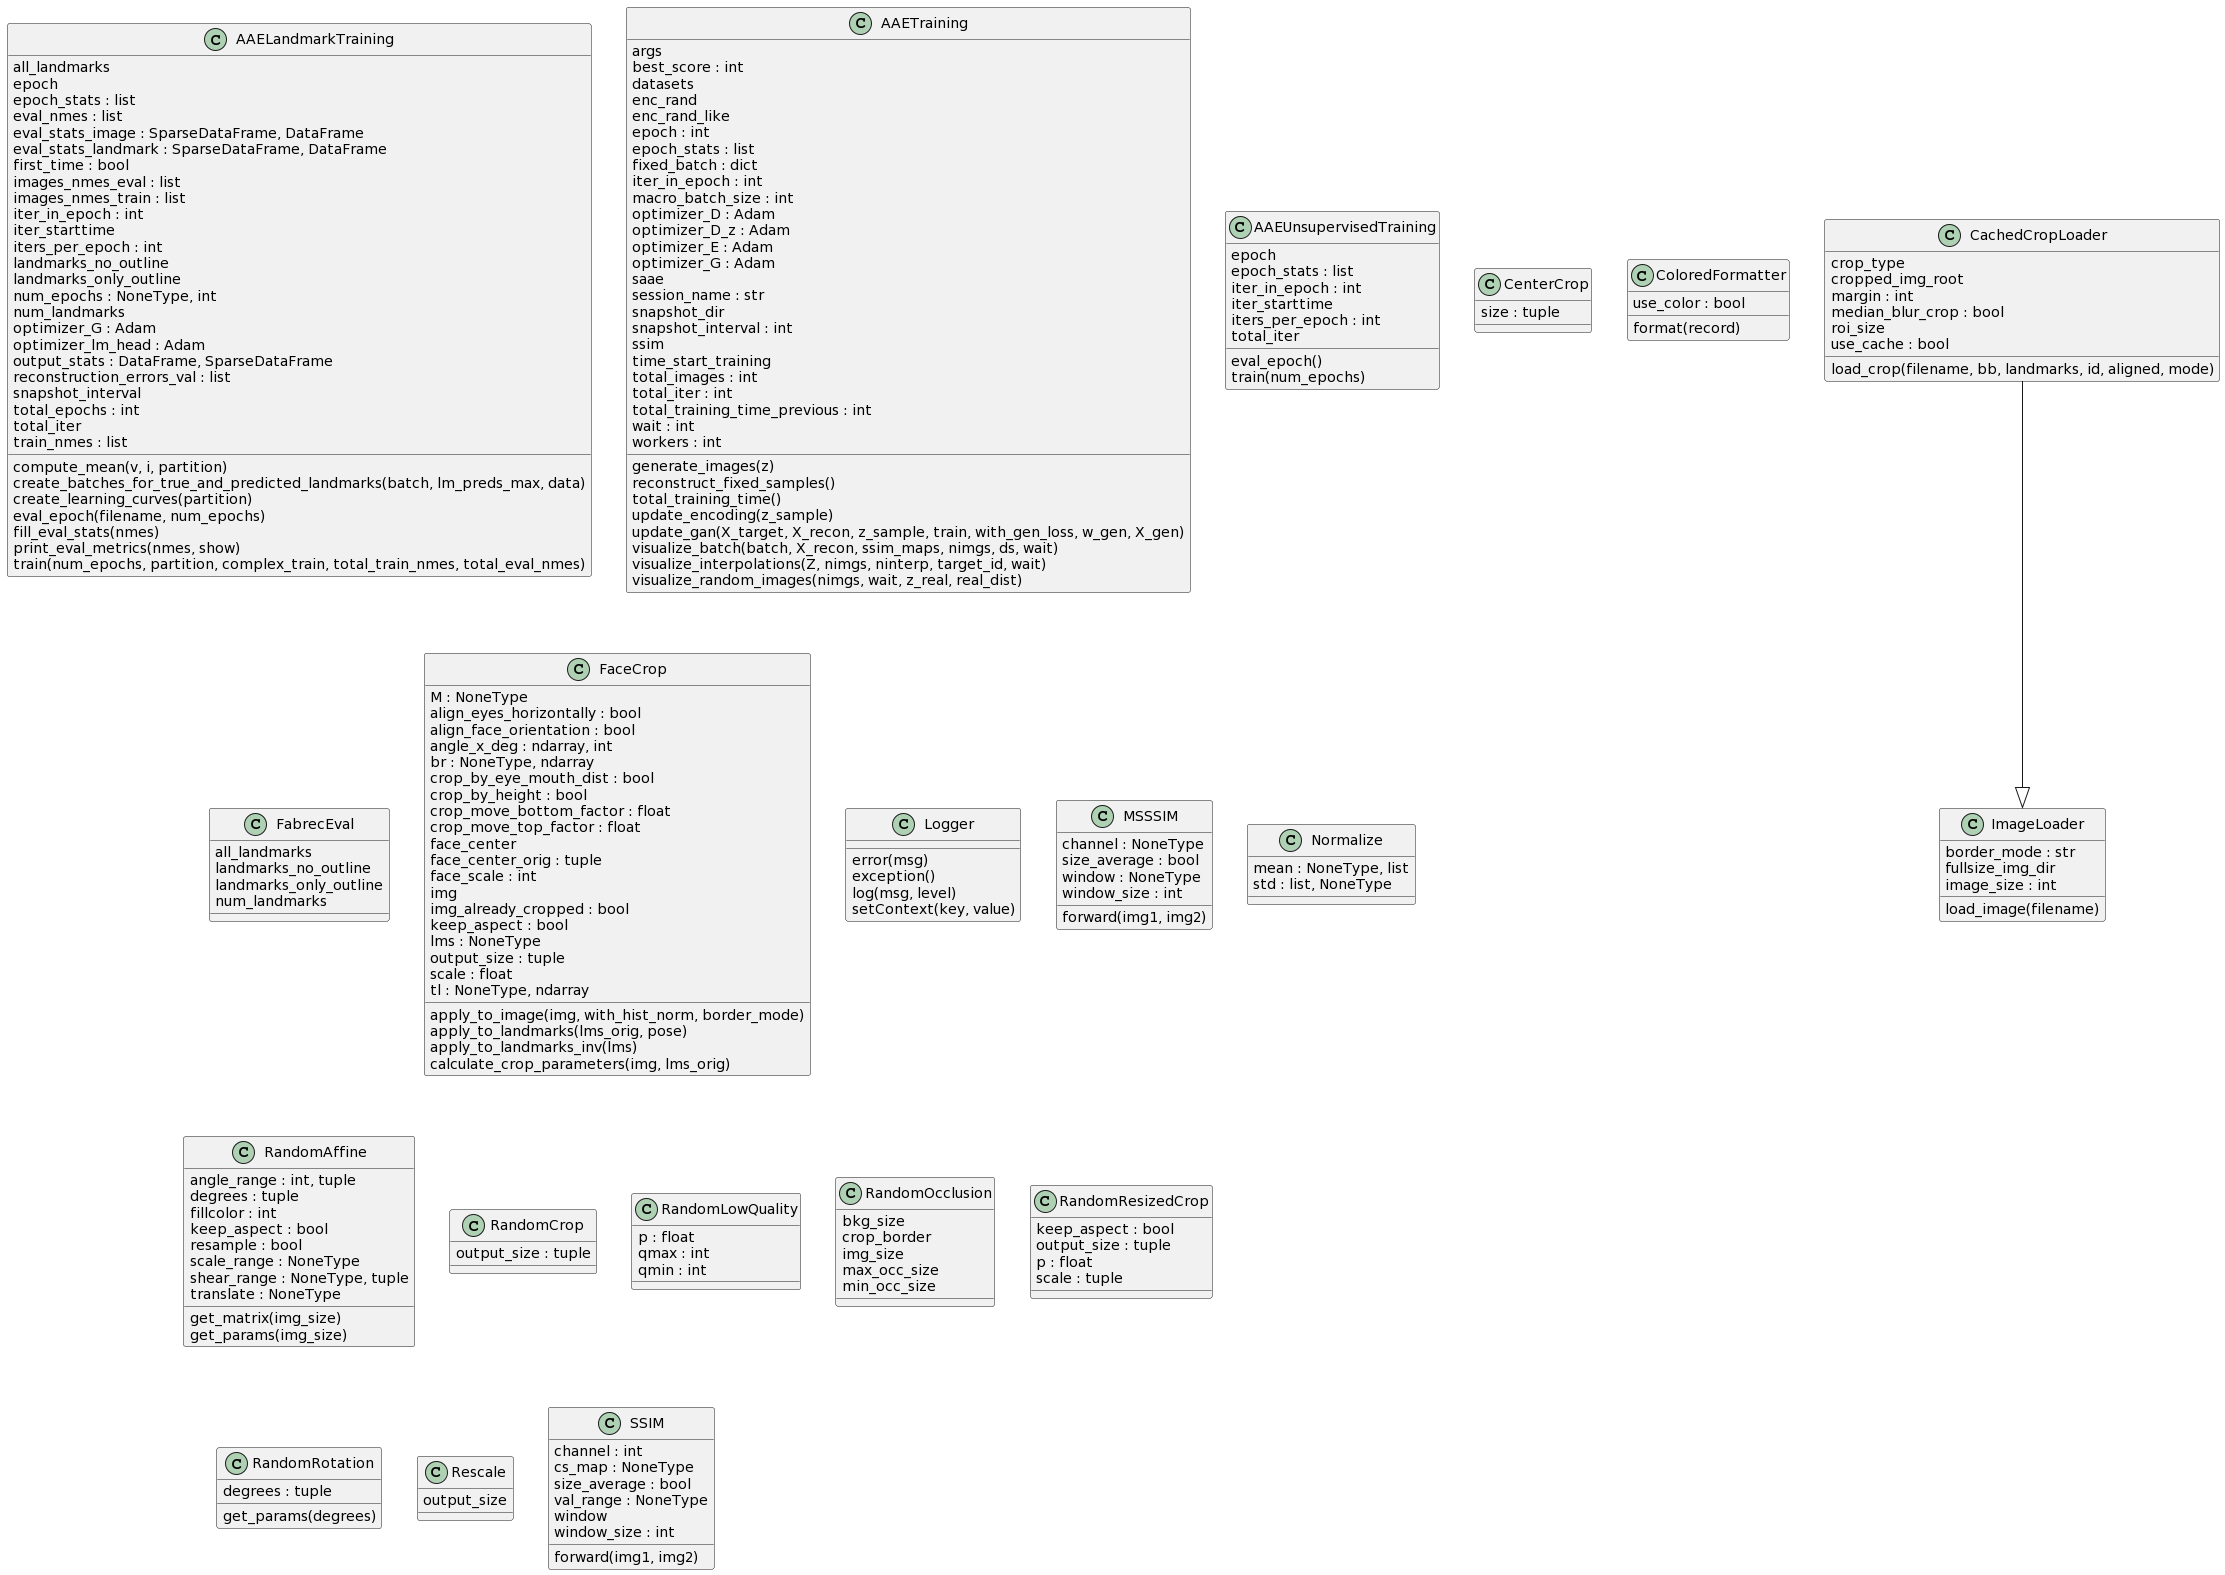
\includegraphics[width=0.99\textwidth]{img/diagrama_clases.png}
    \caption{Diagrama de clases con las principales clases del proyecto.}
    \label{fig:Diagrama_clases}
\end{figure}

\begin{table}[!h]
    \centering
    \caption{Argumentos con los que se ha experimentado en la ejecución del fichero train-aae-landmarks.py}
    \begin{tabular}{|l|l|l|}
    \hline
        Parámetro & Descripción & Valor por defecto \\ \hline
        --train-encoder & Si es True reentrena el encoder & False \\ \hline
        --train-dencoder & Si True reentrena el dencoder & False \\ \hline
        --epochs & Número de épocas que queremos entrenar la red & None \\ \hline
        --batchsize & Tamaño del batchsize para entrenamiento & 50 \\ \hline
        --batchsize-eval & Valor del batchsize para validación & 10 \\ \hline
        --lr & Learning rate para el autoencoder & 0.00002 \\ \hline
        --lr-heatmaps & Learning rate para las ITLs & 0.001 \\ \hline
        --beta1 & Valor de beta 1 para Adam & 0.0 \\ \hline
        --beta2 & Valor de beta 2 para Adam & 0.999 \\ \hline
        --save-freq & Frecuencia de snapshot (en épocas) & 1 \\ \hline
        --dataset & Dataset que se empleará & W300 \\ \hline
        --sigma & Tamaño de los heatmaps & 7 \\ \hline
    \end{tabular}
    \label{table:Params}
\end{table}

\medskip

\noindent Por otro lado, en la \autoref{fig:Diagrama_secuencia} podemos ver el diagrama de secuencia de la ejecución del software 3FabRec para la etapa de entrenamiento y validación y posteriormente para la de evaluación del modelo final. No obstante, remarcamos el hecho de que el software diseñado no tiene como fin su uso por parte de terceros. De ser así, se habría creado una interfaz de usuario amigable en la cual, de manera intuitiva se pudieran elegir las distintas opciones de ejecución.

\newpage

\begin{figure}[!h]
    \centering
    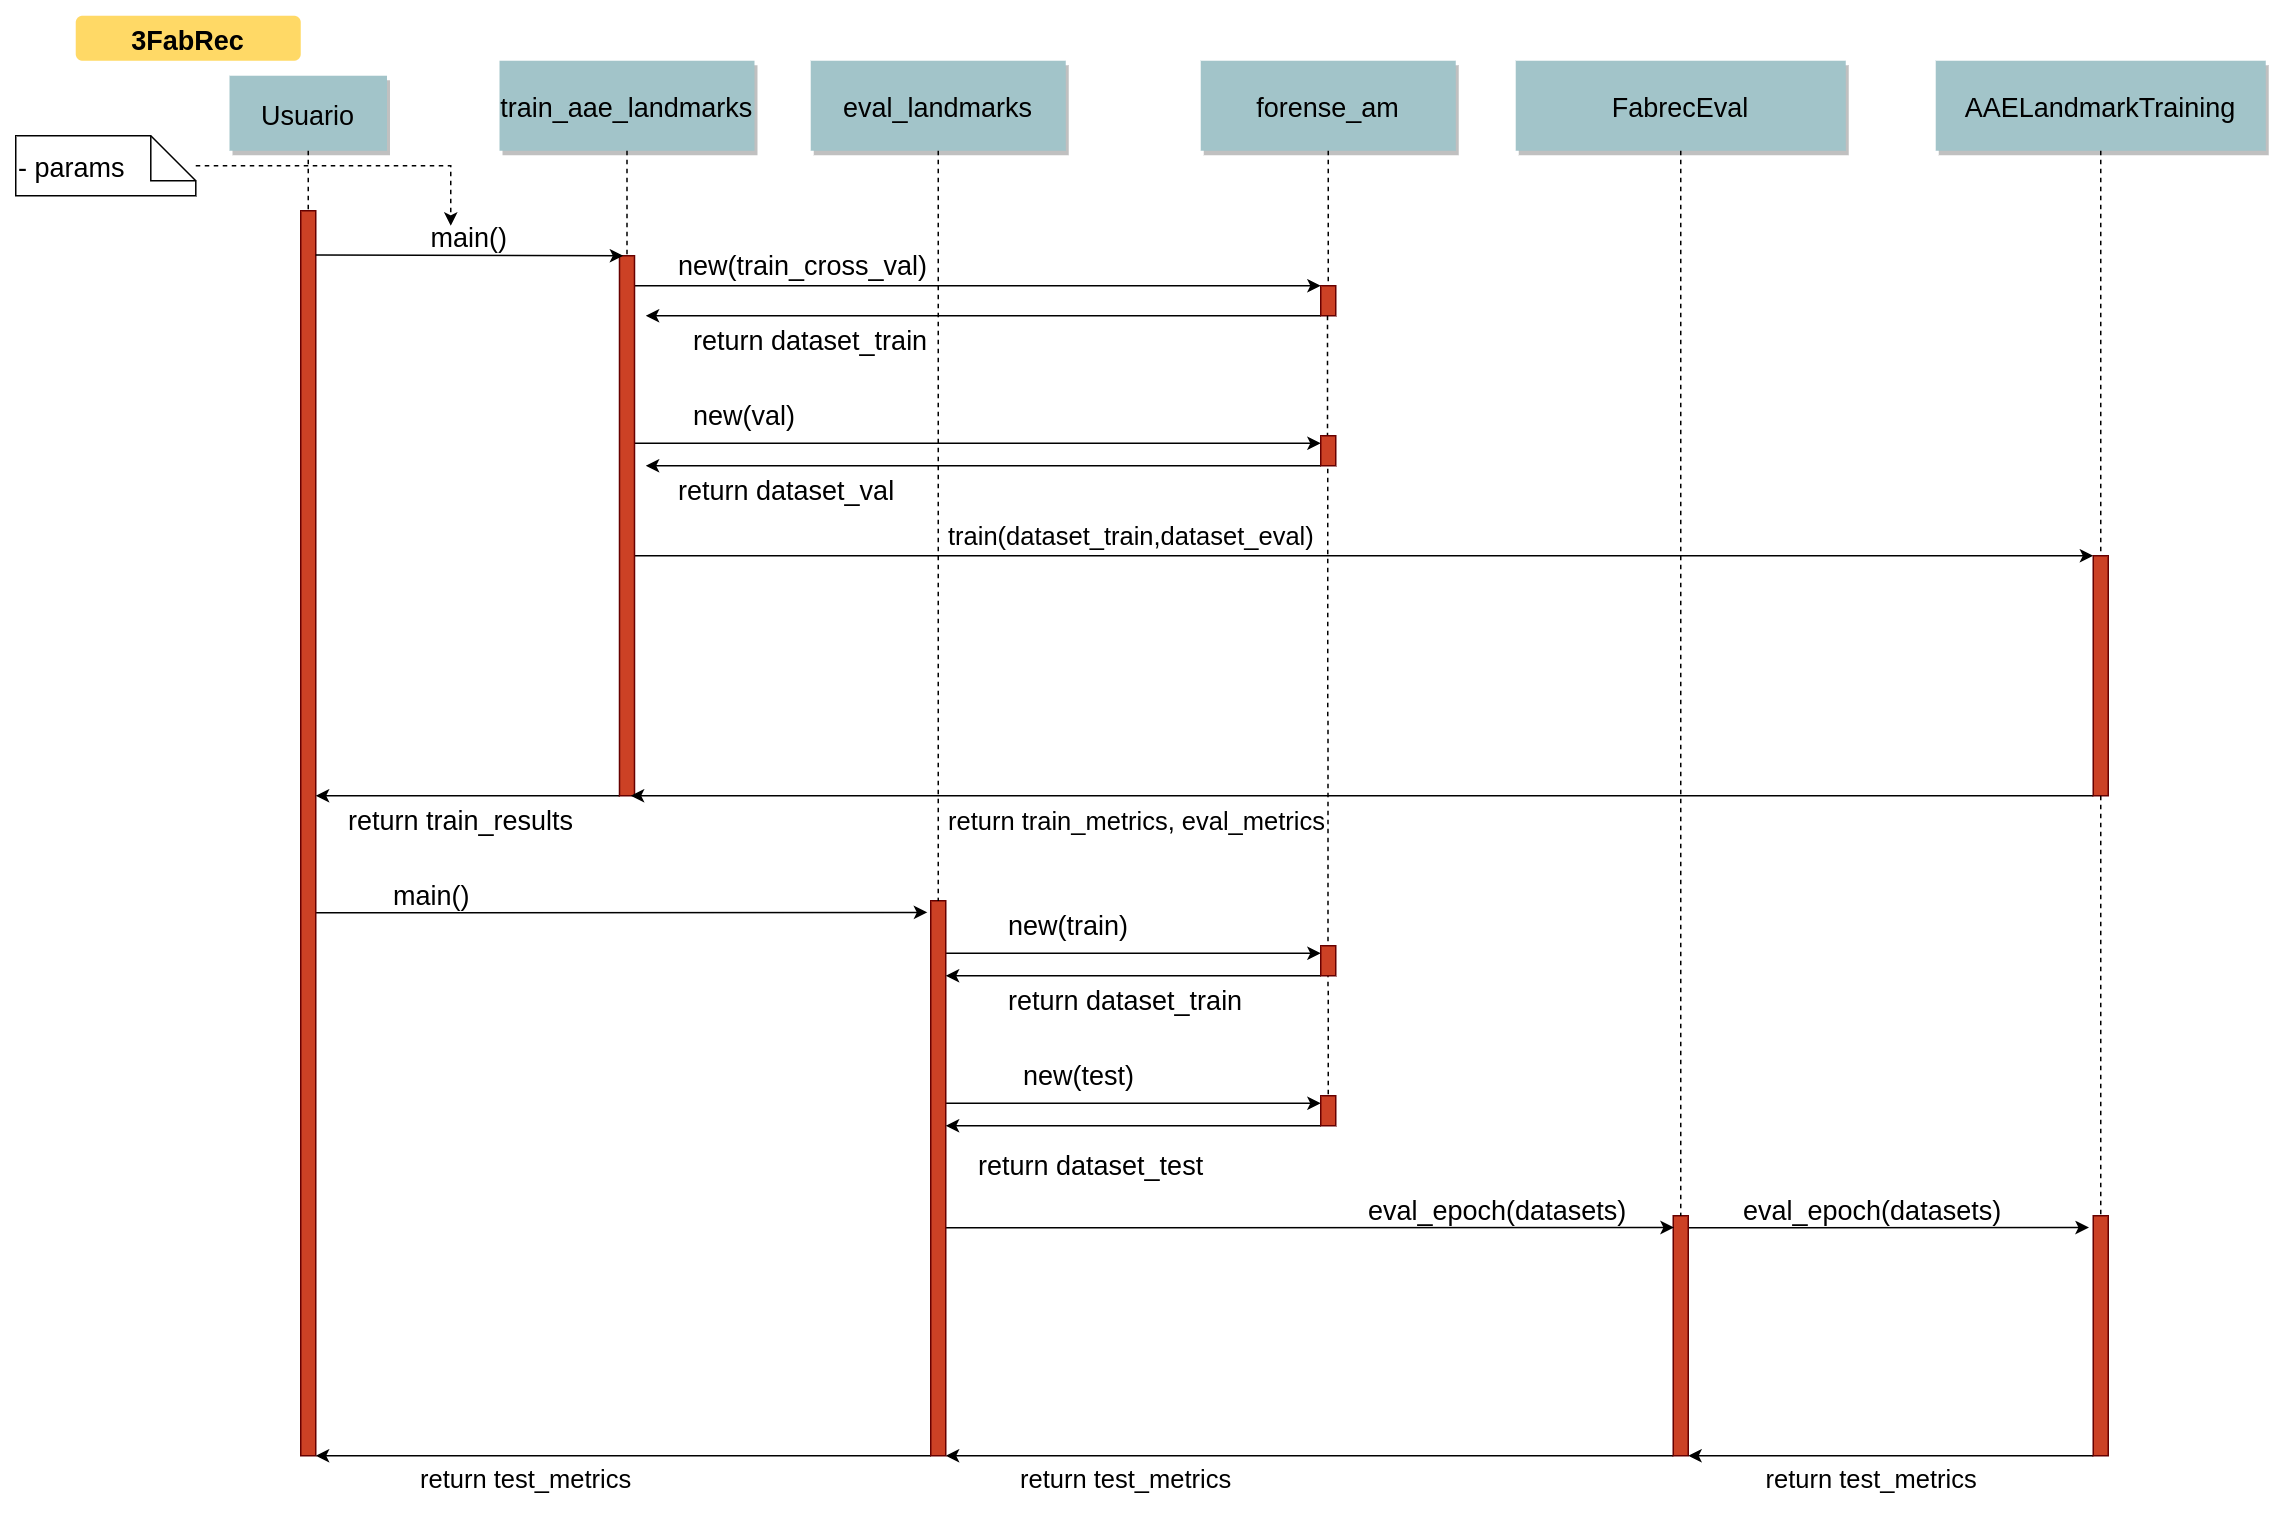
\includegraphics[width=0.99\textwidth]{img/Diagrama_secuencia.png}
    \caption{Diagrama de secuencia del software empleado.}
    \label{fig:Diagrama_secuencia}
\end{figure}

\newpage


\section{Entorno de ejecución}
\noindent Las ejecuciones se han realizado todas en un ordenador portátil \textit{HP Pavilion} con las siguientes características: 

\begin{itemize}
    \item Ubuntu $20.04.5$ LTS $64$ bits.
    \item $8$ GB de RAM
    \item $8$ x Intel® Core™ i$5$-$8300$H CPU @ $2.30$GHz
    \item GPU NVIDIA GeForce GTX $1050$ Mobile
\end{itemize}

\medskip

\noindent Por otro lado, las versiones del software empleado son: 

\begin{itemize}
    \item Python 3.6.13
    \item CUDA 10.1
    \item PyTorch 1.1.0
    \item Numpy 1.17.4
    \item Pandas 0.23.3
    \item Matplotlib 3.3.4
\end{itemize}


\endinput
%------------------------------------------------------------------------------------
% FIN DEL CAPÍTULO. 
%------------------------------------------------------------------------------------

